\documentclass[aspectratio=169]{beamer}
\usepackage{amsmath, amssymb, amsfonts, amsthm}
\usepackage{cancel}
\usepackage[output-complex-root=j]{siunitx}
\usepackage[american, nooldvoltagedirection]{circuitikz}
\usepackage{bm}
\usepackage{listings}
\usepackage{graphicx}
\usepackage{hyperref}

\usetheme{Berkeley}
\usefonttheme[onlymath]{serif}
\AtBeginSection[]{
    \begin{frame}
    \vfill
    \centering
    \begin{beamercolorbox}[sep=8pt,center,shadow=false,rounded=false]{title}
    \usebeamerfont{title}\insertsectionhead\par
    \end{beamercolorbox}
    \vfill
    \end{frame}
}

\newcommand{\N}{\mathbb{N}}
\newcommand{\Z}{\mathbb{Z}}
\newcommand{\Q}{\mathbb{Q}}
\newcommand{\R}{\mathbb{R}}
\newcommand{\C}{\mathbb{C}}
\newcommand{\uvec}[1]{\bm{\hat{#1}}}
\newcommand{\iprod}[2]{\left\langle #1, #2 \right\rangle}
\newcommand{\tpose}[1]{\left[#1\right]^{\! \top} \!\!}
\newcommand{\diff}[1]{\frac{d}{d #1}}

\title{EECS 16B CSM}
\author{Bryan Ngo}
\date{2022-02-15}
\institute{UC Berkeley}

\begin{document}

\begin{frame}
    \maketitle
\end{frame}

\begin{frame}
    \frametitle{Logistics}

    \begin{itemize}
        \item fill out temperature check
        \item pertinent facts
    \end{itemize}

    \includegraphics[width=0.4\textwidth]{pulse.png}
\end{frame}

\begin{frame}
    \tableofcontents
\end{frame}

\section{Change of Basis}

\begin{frame}
    \frametitle{Motivation}

    \begin{columns}
        \column[]{0.5\textwidth}
        \begin{itemize}
            \item conversion from one linear coordinate system to another
            \item \href{https://youtu.be/P2LTAUO1TdA?list=PLZHQObOWTQDPD3MizzM2xVFitgF8hE_ab}{3Blue1Brown video}
        \end{itemize}

        \column[]{0.5\textwidth}
        \includegraphics[width=0.5\textheight]{800px-3d_two_bases_same_vector.svg.png}
    \end{columns}
\end{frame}

\begin{frame}
    \frametitle{A Visualization}

    \begin{center}
        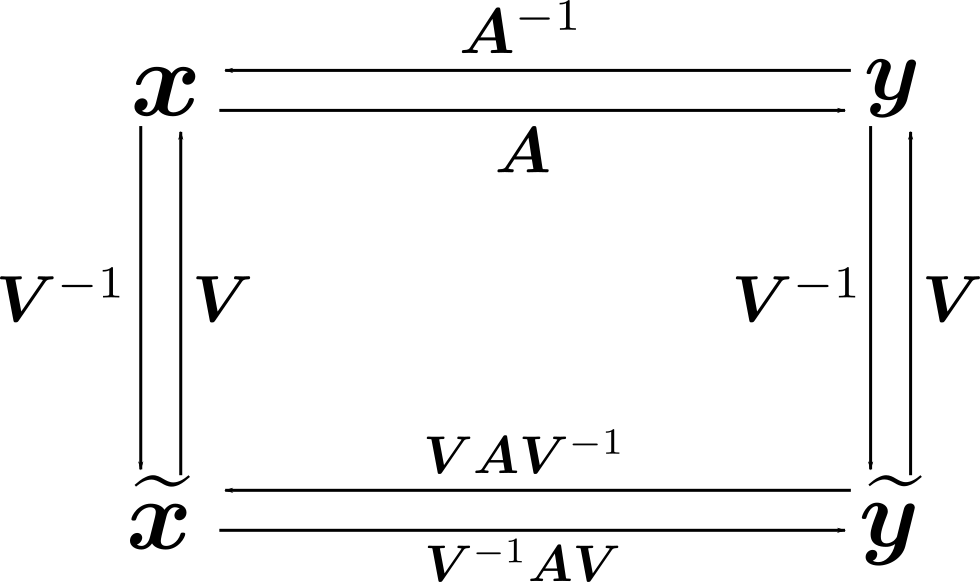
\includegraphics[width=0.8\textwidth]{change-of-basis.png}
    \end{center}
\end{frame}

\begin{frame}
    \frametitle{Diagonalization}

    \begin{itemize}
        \item want the eigenvectors to be the basis for a vector space
        \item makes math \emph{way} easier
    \end{itemize} \pause
    \begin{align}
        \bm{V} &=
        \begin{bmatrix}
            \bm{v}_1 & \bm{v}_2 & \cdots & \bm{v}_n \\
        \end{bmatrix} \\
        \bm{AV} &=
        \begin{bmatrix}
            \lambda_1 \bm{v}_1 & \lambda_2 \bm{v}_2 & \cdots & \lambda_n \bm{v}_n \\
        \end{bmatrix} \\
        &=
        \begin{bmatrix}
            \bm{v}_1 & \bm{v}_2 & \cdots & \bm{v}_n \\
        \end{bmatrix}
        \begin{bmatrix}
            \lambda_1 & 0 & \cdots & 0 \\
            0 & \lambda_2 & \cdots & 0 \\
            \vdots & \vdots & \ddots & \vdots \\
            0 & 0 & \cdots & \lambda_n
        \end{bmatrix} \\
        &= \bm{V \Lambda} \implies \bm{\Lambda} = \bm{V}^{-1} \bm{AV}
    \end{align}
\end{frame}

\section{Inductors}

\begin{frame}
    \frametitle{Basic Properties}

    \begin{center}
        \begin{circuitikz}\draw
            (0, 2) to[L=\(L\), v=\(V_L\), i>^=\(I_L\)] (0, 0)
        ;\end{circuitikz}
    \end{center}
    \begin{equation}
        V_L = L \diff{t} I_L
    \end{equation}
    \begin{itemize}
        \item like a capacitor but for magnetic fields
        \item resists instantaneous change in current \pause
        \item what happens when \(\omega = 0\)? \(\omega = \infty\)?
    \end{itemize}
\end{frame}

\section{Complex Numbers}

\begin{frame}
    \frametitle{Definition}

    \begin{equation}
        z = \underbrace{a + bj}_{\text{rectangular}} = \underbrace{r e^{j \theta}}_{\text{polar}}
    \end{equation}
    \begin{itemize}
        \item \(a, b, r, \theta \in \R\)
        \item \(j^2 = -1\)
        \item we use \(j\) in EE
    \end{itemize}
\end{frame}

\begin{frame}
    \frametitle{Coordinate Transforms}

    \begin{align}
        r^2 &= a^2 + b^2 \\
        \tan(\theta) &= \frac{b}{a} \\
        a &= \Re\{z\} = r \cos(\theta) \\
        b &= \Im\{z\} = r \sin(\theta)
    \end{align}
\end{frame}

\begin{frame}
    \frametitle{Euler's Formula}

    \begin{equation}
        e^{j \theta} = \cos(\theta) + j \sin(\theta)
    \end{equation}
    \begin{itemize}
        \item \href{https://youtu.be/v0YEaeIClKY}{relevant 3Blue1Brown}
        \item \(e^{j \pi} + 1 = 0\) is a special case
    \end{itemize}
\end{frame}

\end{document}
